\clearpage
\graphicspath{{./lib/parameter_estimation/figures/}}
\section{Parameter Estimation}

\begin{tcolorbox}	
	\begin{tabular}{p{2.75cm} p{0.2cm} p{10.5cm}} 	
        \textbf{Header Files}    &:& parameter\_estimation\_*.h \\
		\textbf{Source Files}    &:& parameter\_estimation\_*.cpp \\
        \textbf{Version}        &:& 20190528 (Andoni Santos)
	\end{tabular}
\end{tcolorbox}

\maketitle
This block is used to estimate the error rate between two sets of data shared
by two parties in Quantum Key Distribution, Alice and Bob. It does this by
randomly sampling a predefined number of bits from the sifted key, exchanging
and comparing them. The error rate of the exchanged bits provides an estimative
of the overall error rate of the sifted key. 

% % \begin{multicols}{3}
% % \begin{enumerate}
% % 	\item Random
% % 	\item PseudoRandom
% % 	\item DeterministicCyclic
% % 	\item DeterministicAppendZeros
% %     \item AsciiFileAppendZeros
% %     \item AsciiFileCyclic
% % \end{enumerate}
% % \end{multicols}

\subsection*{Signals}

\begin{table}[h]
	%\centering
	\begin{tabular}{|c|l|}
		\hline
		\textbf{Number of Input Signals} & 2 \\ \hline
        \textbf{Type of Input Signals} & Binary, TimeDiscreteAmplitudeContinuousReal \\ \hline
    	\textbf{Number of Output Signals} & 3 \ \\ \hline
        \textbf{Type of Output Signals} & Binary,
		TimeDiscreteAmplitudeContinuousReal,\\
		& TimeDiscreteAmplitudeContinuousReal \\ \hline
	\end{tabular}
	\caption{Parameter estimation signals}
	\label{table:par_est_signals}
\end{table}

\subsection*{Input Parameters}

%	\begin{itemize}
%		\item mode\{PseudoRandom\}\linebreak
%		(Random, PseudoRandom, DeterministicCyclic, DeterministicAppendZeros)
%		\item probabilityOfZero\{0.5\}\linebreak
%		(real $\in$ [0,1])
%		\item patternLength\{7\} \linebreak
%		(integer $\in$ [1,32])
%		\item bitStream\{"0100011101010101"\} \linebreak
%		(string of 0's and 1's)
%		\item numberOfBits\{-1\} \linebreak
%		(long int)
%		\item bitPeriod\{1.0/100e9\} \linebreak
%		(double)
%	\end{itemize}

\begin{table}[h]
	\centering
	\begin{tabular}{|c|c|p{60mm}|c|ccp{60mm}}
		\cline{1-4}
		\textbf{Parameter} & \textbf{Type} & \textbf{Values} &   \textbf{Default}& \\ \cline{1-4}
		alpha & t\_real & [0,1] & 0.05 \\ \cline{1-4}
		numberOfBits & t\_integer & > 1 & 500 \\ \cline{1-4}
		numberOfBitsRequiredToStart & t\_integer &  > numberOfBits & 10500 \\ \cline{1-4}
		threshold & t\_real & [0,1] & 0.12 \\ \cline{1-4}
		bypassParameterEstimation & bool & [true, false] & false \\ \cline{1-4}
	\end{tabular}
	\caption{Parameter estimation input parameters}
	\label{table:par_est_in_par}
\end{table}

\subsection*{Methods}
\bigbreak	
ParameterEstimation(initializer\_list<Signal*> InputSig, initializer\_list<Signal*> OutputSig)
\bigbreak	
ParameterEstimation(initializer\_list<Signal*> InputSig,
initializer\_list<Signal*> OutputSig, string bFolderName)
\bigbreak	
ParameterEstimation(initializer\_list<Signal*> InputSig, initializer\_list<Signal*> OutputSig, string bFolderName, string bFileName)
\bigbreak	
ParameterEstimation(initializer\_list<Signal*> InputSig,
initializer\_list<Signal*> OutputSig, string bFolderName, string bFileName,
string bLFileName)
\bigbreak
void initialize(void);
\bigbreak	
bool runBlock(void);
\bigbreak
void setConfidence(double P)
\bigbreak
double const getConfidence(void)
\bigbreak
void setNumberOfBitsToUse(const unsigned int nb)
\bigbreak
void setNumberOfBitsRequiredToStart(const unsigned int nbs)
\bigbreak
void setBypassParameterEstimation(const bool bypass)
\bigbreak
void setParameterEstimationRole(const parameter\_estimation\_role role)
\bigbreak
void setThreshold(const t\_real thr)
\bigbreak
long int getInputBits(void)
\bigbreak
long int getOutputBits(void)
\bigbreak
t\_real getAverageEstimatedBER(void)
\bigbreak

\subsection*{Functional description}

This block estimates the error rate between sifted keys held by two different
parties, while sharing only a relatively small random subset of the keys. This
keeps most of the data away from the communication channels. The small
amount of shared data is discarded afterwards to maintain the privacy of the
remaining data.

Let's assume that, for instance, in a Quantum Key Distribution protocol, there
are two parties who want to generate a shared private key. These two parties are
Alice, who transmits the data, and Bob, who receives the data. At a certain
point, they both have sifted keys, where both have the data corresponding to the
qubits which Bob correctly received and measured. However, the sifted keys are
still not equal, as they are affected by transmission errors. These errors can
be due to multiple reasons, the most important of which is attempted
interference by a third party. Thus, it becomes necessary to estimate the error
rate for two reasons:

\begin{enumerate}
	\item Estimate the potential amount of data which has been intercepted, to
	find if it is possible to distill a secure key, and how much of the key may
	have been compromised;
	\item Choose the parameters to efficiently correct the errors, minimizing
	the amount of data that will need to be discarded in the process.
\end{enumerate}

To do this, some data needs to be shared between Alice and Bob, and that data
will be compromised. Therefore, the amount of shared data should be minimized,
as it will have to be discarded afterwards. This is currently done as follows.

The \textit{ParameterEstimation} block receives the binary sifted keys in a
queue. After Bob has accumulated enough bits, as defined by
\textit{numberOfBitsRequiredToStart}, it starts the parameter estimation
process. First, it generates a random seed, which will be used to seed a random
generator. This generator will randomly choose \textit{numberOfBits} among the
first \textit{numberOfBitsRequiredToStart} bits in the queue. Then, it will send
the seed and the bits themselves to Alice. Alice can then sample the same bits
and compare them to Bob's. The ratio between the number of coincidences and
\textit{numberOfBits} provides an estimate to the overall error rate in the
accumulated \textit{numberOfBitsRequiredToStart}. Alice then sends the bits
information to Bob, outputs the accumulated \textit{numberOfBitsRequiredToStart}
(except for the shared bits), and the remaining other signals it sends the upper
bound of the BER confidence interval and the total number of remaining bits.
Bob then receives the data sent by Alice, get its own estimate and outputs the
same data.

% \subsection*{Input Signals}


% \subparagraph*{Number:} 0

% \subparagraph*{Type:} Binary (DiscreteTimeDiscreteAmplitude)

% \subsection*{Output Signals}

% \subparagraph*{Number:} 1 or more

% \subparagraph*{Type:} Binary (DiscreteTimeDiscreteAmplitude)

% \subsection*{Illustrative Examples}

% \paragraph*{Random Mode}

% \paragraph*{PseudoRandom Mode}
% Consider a pseudorandom sequence with \textit{patternLength}=3 which contains a total of 7 ($2^3-1$) bits. In this sequence it is possible to find every combination of 0's and 1's that compose a 3 bit long subsequence with the exception of $000$. For this example the possible subsequences are $010$, $110$, $101$, $100$, $111$, $001$ and $100$ (they appear in figure \ref{BinarySequenceN3} numbered in this order). Some of these require wrap.

% % \begin{figure}[h]
% % 	\centering
% % 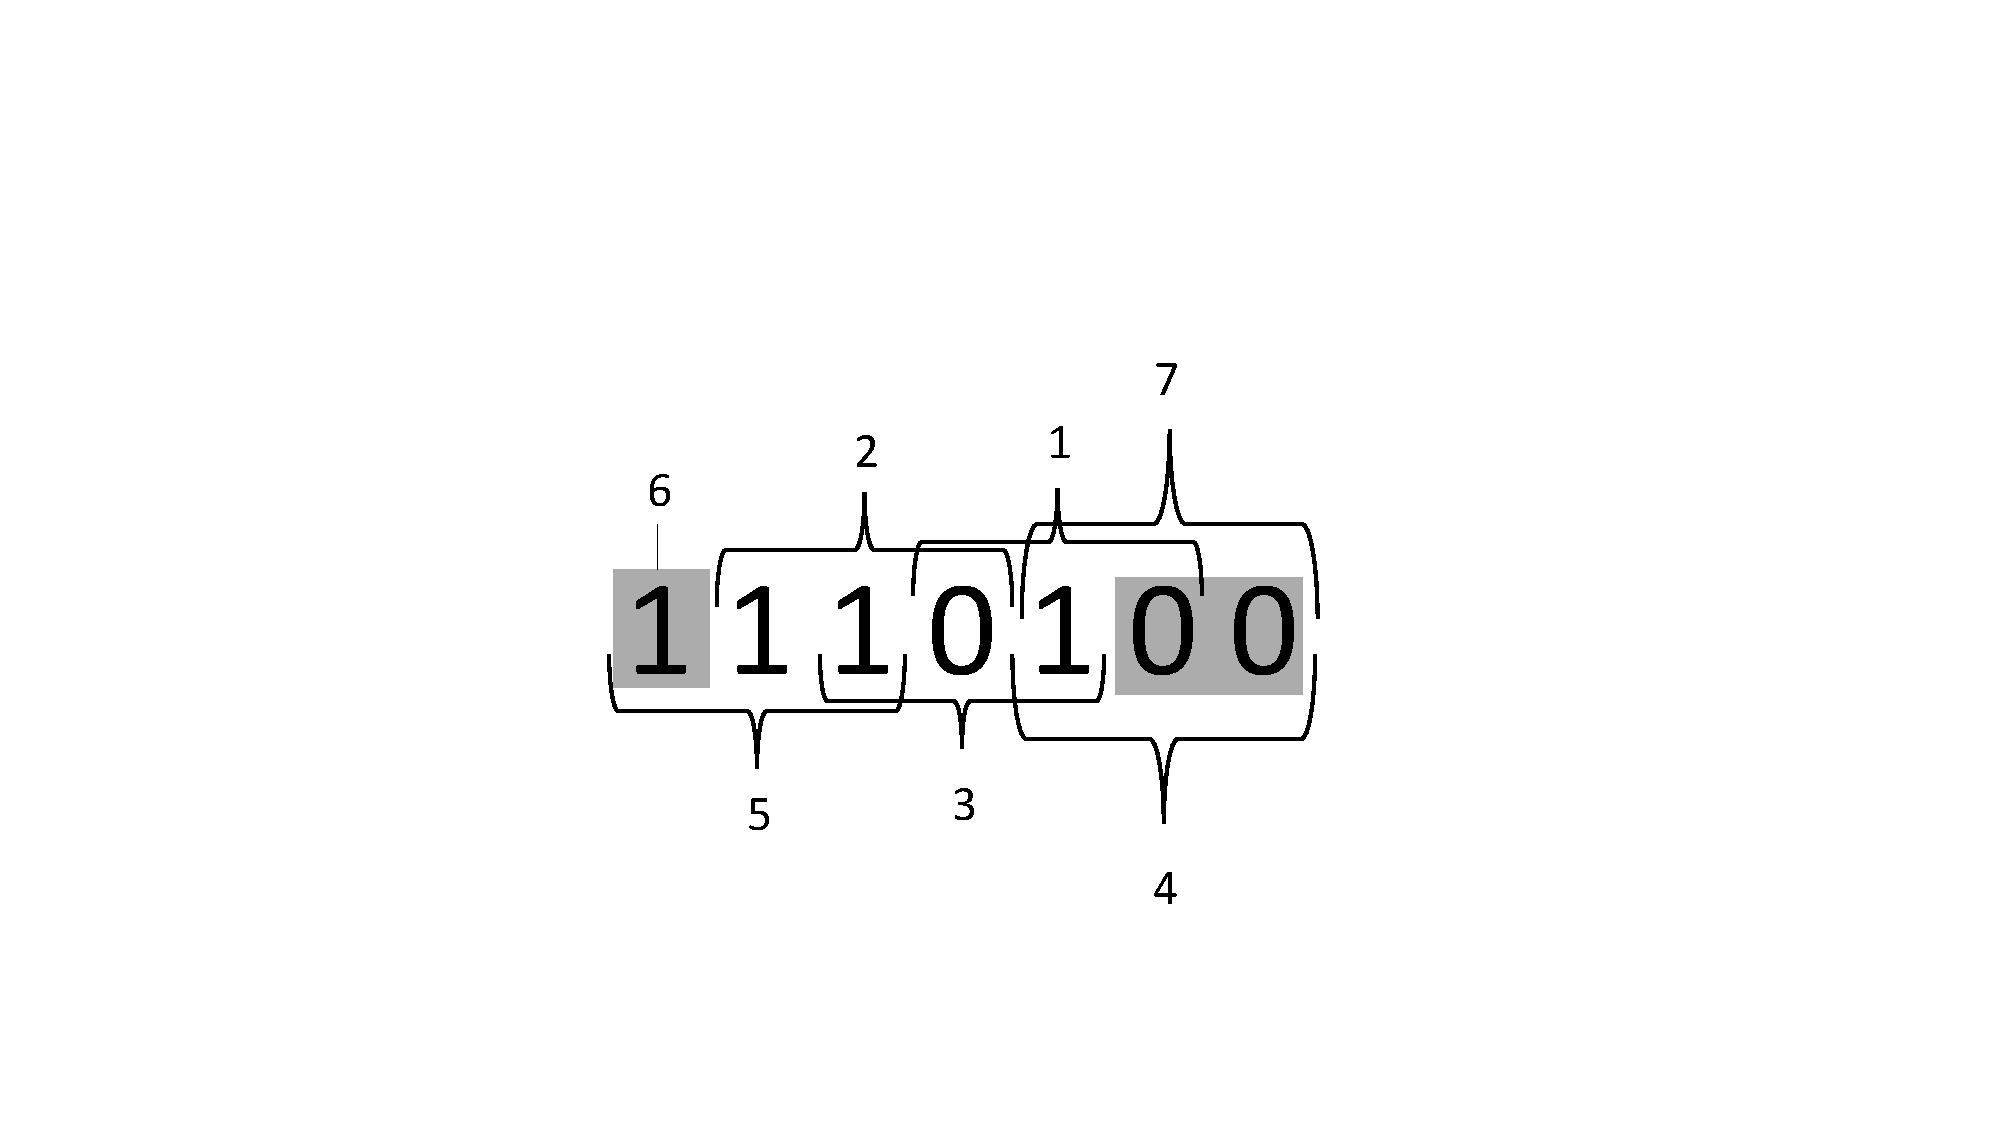
\includegraphics[width=\textwidth]{BinarySequenceN3.pdf}
% % \caption{Example of a pseudorandom sequence with a pattern length equal to 3.}\label{BinarySequenceN3}
% % \end{figure}

% \paragraph*{DeterministicCyclic Mode}

% Take the \textit{bit stream} '0100011101010101'. The generated binary signal is displayed in.

% \paragraph*{DeterministicAppendZeros Mode}

% Take the \textit{bit stream} '0100011101010101'. The generated binary signal is displayed in \ref{MQAM1_DeterministAppendZeros}.

% % \begin{figure}
% % 	\centering
% % 	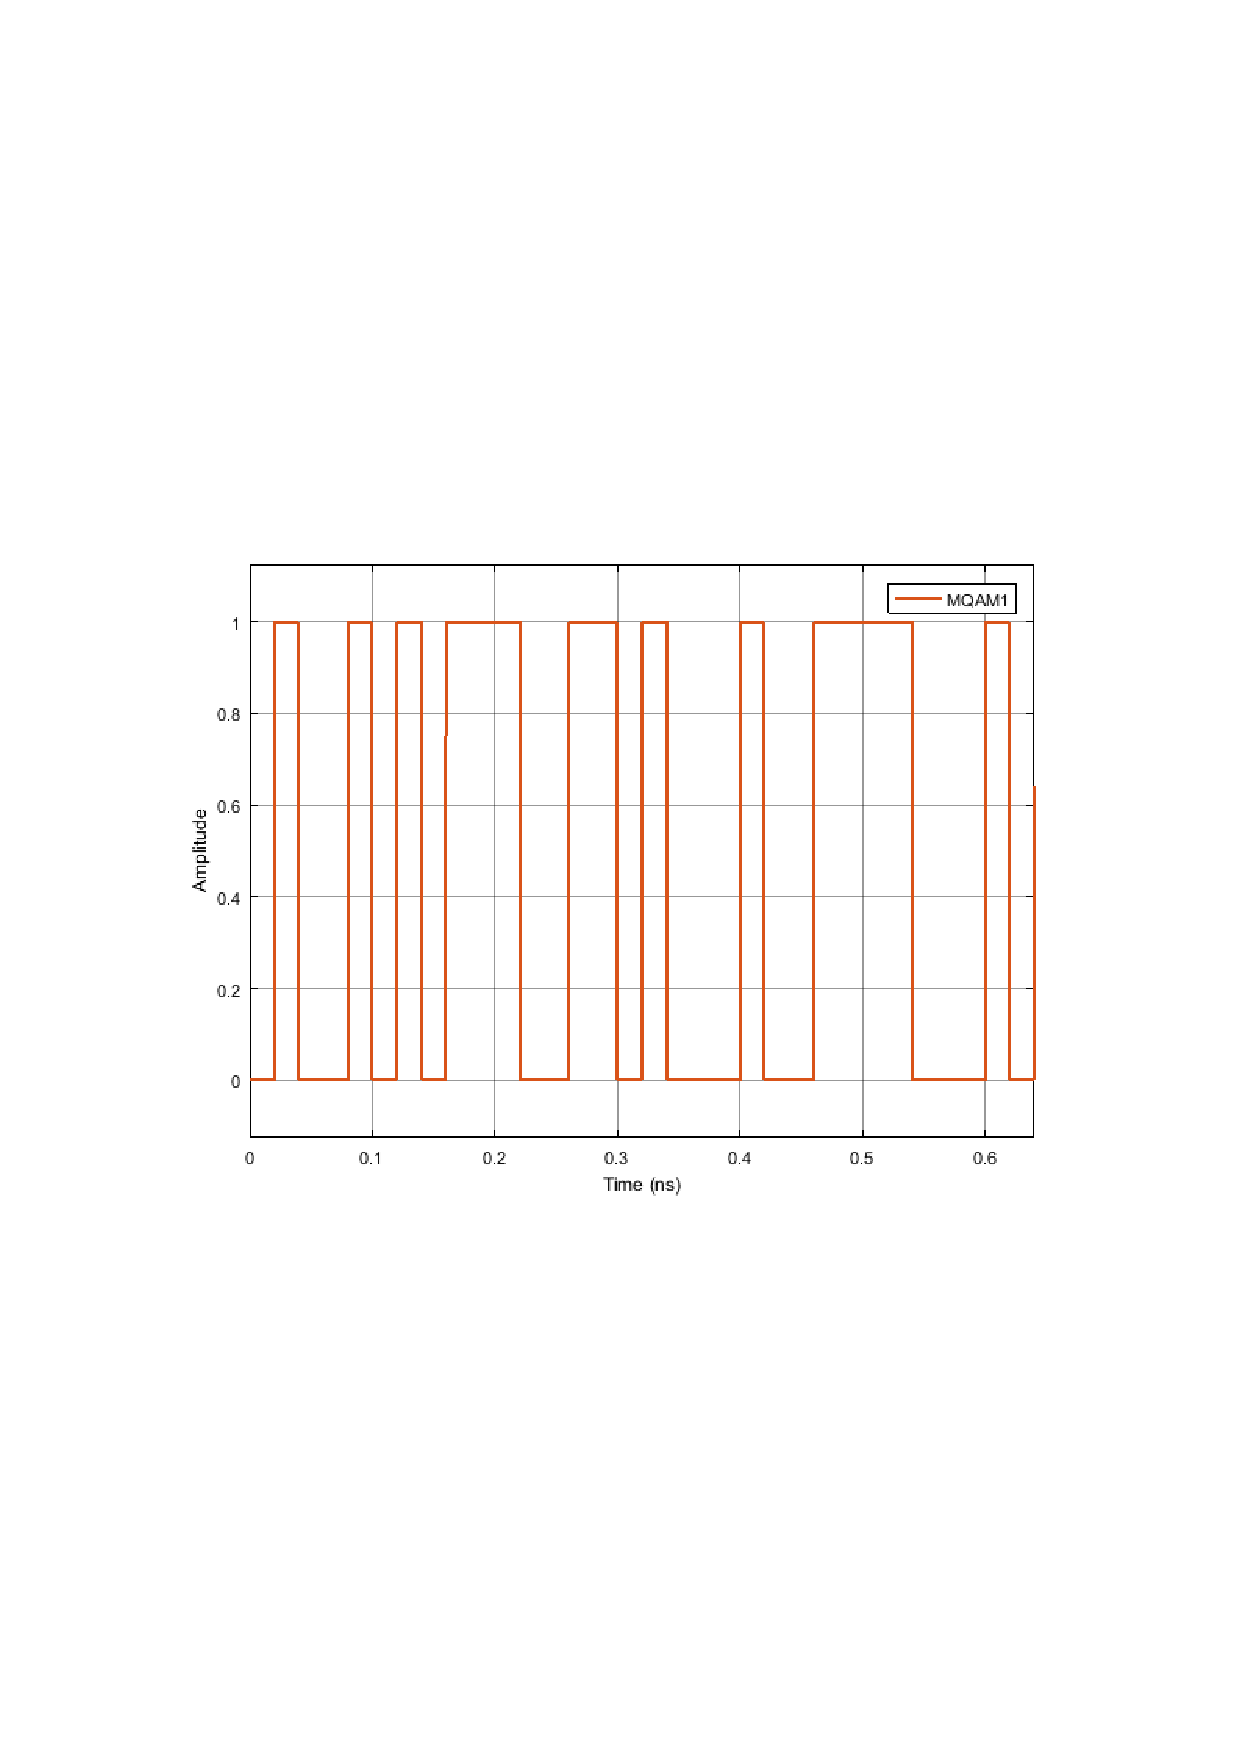
\includegraphics[clip, trim=0.5cm 9cm 0.5cm 9cm, width=\textwidth]{BinarySource_output.pdf}
	
% % 	\caption{Binary signal generated by the block operating in the \textit{Deterministic Append Zeros} mode with a binary sequence 01000...}\label{MQAM1_DeterministAppendZeros}
% % \end{figure}

\subsection*{Suggestions for future improvement}

% Currently, the number and type of signals is fixed, and cannot easily be
% adapted. In the future, this could be changed to allow easily adapting the
% message processors to other situations. In order to do that, it should be
% possible to choose a given number of signals and define the desired type for
% each of them.

